% Provenance (never printed): cycle 3 / 6e "La planete Terre" (structure of
% the globe: crust, mantle, core); see sources/book1/PROVENANCE.md. Book 1,
% grade 6, chapter 4.
% Vocabulary guard: "magma" not before g7.2 ("molten rock"); P and S waves,
% Moho, core--mantle boundary and lithosphere belong to Book 2 (g11): the
% waves are told in prose, never defined; "seismometer" is defined in g7.3.
\chapter{Bagian Dalam Bumi}\label{ch:g6:inside-the-earth}

Di ujung barat laut Rusia, tidak jauh dari perbatasan dengan Norwegia,
sebuah tutup logam dilas ke tanah di antara bangunan-bangunan yang
ditinggalkan. Di bawahnya, sebuah lubang yang lebarnya hanya kira-kira
23~sentimeter menembus lurus ke bawah sedalam lebih dari 12~kilometer:
itulah lubang terdalam yang pernah digali. Pengeborannya memakan waktu
kira-kira 20~tahun. Para pengebor berharap dapat menggali lebih dalam lagi,
tetapi di dasarnya suhu \omterm{def:g3:stones-pebbles-sand:rock}{batuan} mencapai kira-kira 180~derajat Celsius,
hampir dua kali lebih panas daripada yang diperkirakan: panas itu
membengkokkan mata bor dan pipa-pipanya, dan pekerjaan dihentikan pada
tahun 1992. Padahal pusat Bumi lebih dari \textbf{500 kali} lebih dalam
daripada dasar lubang itu. Bagaimana kita dapat mengetahui apa yang ada di
bawah sana?
% ledger: sciam:kola-depth, sciam:kola-180C, earth:Rmean

\begin{omfigure}
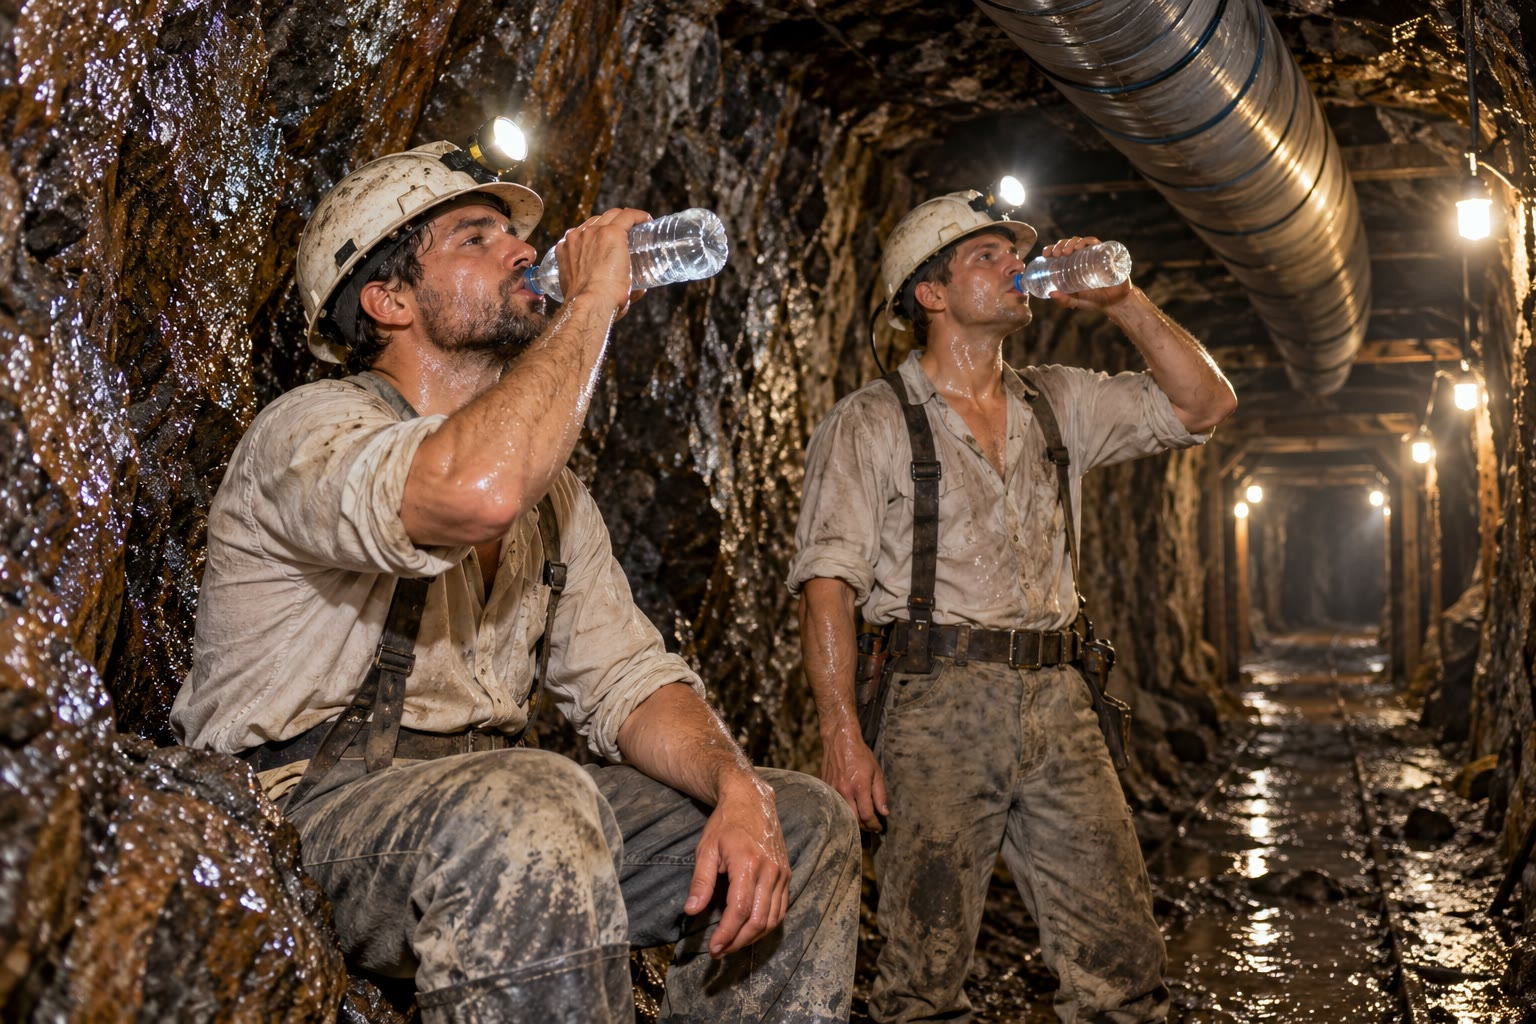
\includegraphics[width=0.62\linewidth]{images/book1/ai/g6-deep-mine.jpg}

{\small Para penambang minum di sebuah lorong tambang yang panas, berkilometer
di bawah tanah. (Ilustrasi AI.)}
\end{omfigure}

\begin{recall}
Bumi adalah \omterm{def:g6:earth-a-planet:planet-types}{planet batuan}, sebuah bola yang lebarnya kira-kira 12\,742~km:
jari-jarinya, dari permukaan sampai ke pusat, kira-kira 6371~km
(\cref{ch:g6:earth-a-planet}). \omterm{def:g3:stones-pebbles-sand:rock}{Batuannya} termasuk dalam tiga keluarga, beku,
sedimen, dan metamorf (\cref{ch:g6:rocks-and-minerals}). Di \omterm{def:g4:volcanoes-earthquakes-first-look:volcano}{gunung api},
\omterm{def:g3:stones-pebbles-sand:rock}{batuan} yang meleleh naik dari bawah dan tercurah keluar sebagai \omterm{def:g4:volcanoes-earthquakes-first-look:eruption}{lava}; ketika
\omterm{def:g4:volcanoes-earthquakes-first-look:earthquake}{gempa bumi}, tanah berguncang (\cref{ch:g4:volcanoes-earthquakes-first-look}).
\end{recall}
% ledger: earth:Rmean

\section{Seberapa dalam kita pernah masuk?}

Sejak lama manusia menggali ke dalam Bumi, untuk mencari air, batu, dan
logam. Ada dua jenis lubang yang paling dalam.

\textbf{Tambang.} Tambang terdalam di dunia adalah tambang emas di dekat
Johannesburg, di Afrika Selatan. Lorong-lorongnya menembus lebih dari 4~km
di bawah permukaan. Di bawah sana, dinding \omterm{def:g3:stones-pebbles-sand:rock}{batuannya} mencapai kira-kira
60~derajat Celsius: tambang itu didinginkan dengan memompakan ribuan ton es
yang dicampur air ke bawah, dan dengan kipas raksasa yang meniupkan udara
melalui lorong-lorongnya.
% ledger: gwr:deepest-mine

\textbf{Lubang bor.} Lubang bor adalah lubang sempit yang dibor dari
permukaan oleh sebuah mesin; tidak ada orang yang turun ke dalamnya. Yang
paling dalam adalah lubang bor dalam cerita pembuka, yang digali untuk
ilmu pengetahuan di Semenanjung Kola, di barat laut Rusia: 12\,262~meter,
yaitu kira-kira 12.3~km.
% ledger: sciam:kola-depth

Kedalaman ini tampak sangat besar. Dibandingkan dengan ukuran Bumi,
kedalaman itu sangat kecil. Gambar di bawah ini menunjukkannya pada satu
jalur, di samping \omterm{def:g1:landscapes-around-us:landform}{gunung} tertinggi, Gunung Everest (8849~m).
% ledger: tht:everest

\begin{omfigure}
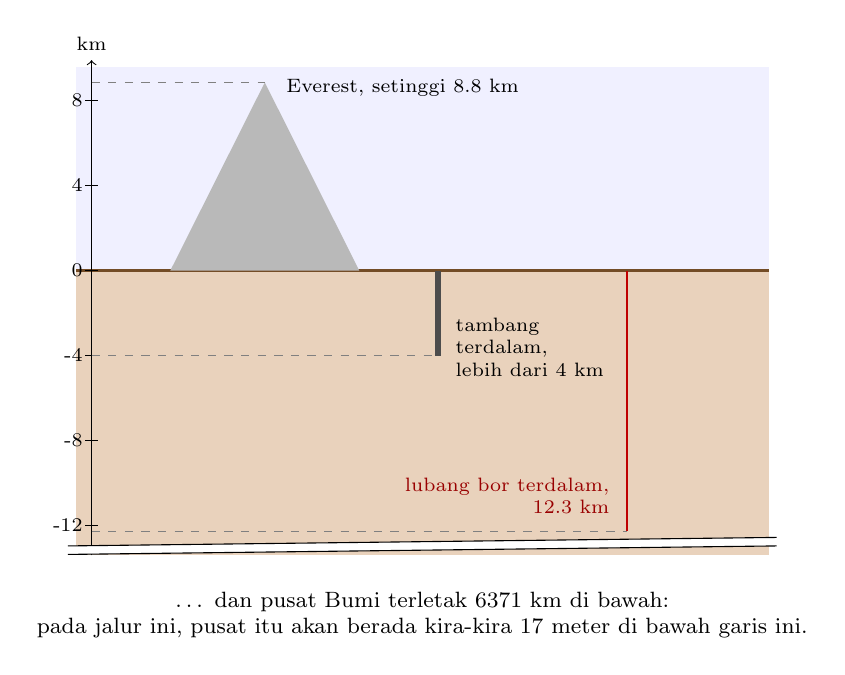
\begin{tikzpicture}[yscale=0.27, xscale=1]
  % sea-level ground and the sky
  \fill[blue!6] (-0.2,0) rectangle (8.6,9.6);
  \fill[brown!35] (-0.2,0) rectangle (8.6,-13.4);
  \draw[thick, brown!60!black] (-0.2,0) -- (8.6,0);
  % depth axis
  \draw[->] (0,-13.4) -- (0,9.9) node[above, font=\scriptsize] {km};
  \foreach \y in {-12,-8,-4,0,4,8} \draw (-0.08,\y) -- (0.08,\y) node[left=2pt, font=\scriptsize] {\y};
  % Everest
  \fill[gray!55] (1.0,0) -- (2.2,8.849) -- (3.4,0) -- cycle;
  \draw[dashed, gray] (0,8.849) -- (2.2,8.849);
  \node[font=\scriptsize, right] at (2.35,8.6) {Everest, setinggi 8.8~km};
  % deepest mine
  \draw[line width=2.2pt, black!70] (4.4,0) -- (4.4,-4);
  \draw[dashed, gray] (0,-4) -- (4.4,-4);
  \node[font=\scriptsize, right, align=left] at (4.5,-3.6) {tambang\\ terdalam,\\ lebih dari 4~km};
  % Kola borehole
  \draw[line width=0.7pt, red!75!black] (6.8,0) -- (6.8,-12.262);
  \draw[dashed, gray] (0,-12.262) -- (6.8,-12.262);
  \node[font=\scriptsize, left, align=right, red!60!black] at (6.7,-10.6) {lubang bor terdalam,\\ 12.3~km};
  % break and the centre
  \draw[white, line width=3pt] (-0.3,-13.15) -- (8.7,-12.75);
  \draw (-0.3,-13.35) -- (8.7,-12.95);
  \draw (-0.3,-12.95) -- (8.7,-12.55);
  \node[font=\footnotesize, align=center] at (4.2,-16.2) {\ldots\ dan pusat Bumi terletak 6371~km di bawah:\\
     pada jalur ini, pusat itu akan berada kira-kira 17~meter di bawah garis ini.};
\end{tikzpicture}

{\small \omterm{def:g4:world-physical-map:altitude}{Ketinggian} dan kedalaman digambar dengan skala yang sama (1~cm untuk
3.7~km), dari \omterm{def:g4:world-physical-map:altitude}{permukaan laut}. Patahan pada jalur menyembunyikan hampir
seluruh perjalanan menuju pusat.}
% ledger: tht:everest, gwr:deepest-mine, sciam:kola-depth, earth:Rmean
\end{omfigure}

\begin{method}[Membandingkan kedalaman dengan jari-jari Bumi]\label{met:g6:inside-the-earth:percent}
\begin{enumerate}
  \item Tuliskan kedalaman dan jari-jari dalam satuan yang sama (kilometer).
  \item Bagilah kedalaman dengan jari-jari, lalu kalikan dengan 100: hasilnya
        adalah kedalaman sebagai persentase dari perjalanan menuju pusat.
  \item Untuk menyatakan berapa kali lebih dalam letak pusat, bagilah
        jari-jari dengan kedalaman.
\end{enumerate}
\end{method}

\begin{example}[Lubang bor terdalam]\label{ex:g6:inside-the-earth:kola}
Lubang bor itu sedalam 12.3~km dan jari-jari Bumi 6371~km.
$12.3 \div 6371 \approx 0.0019$, dan $0.0019 \times 100 = 0.19$: lubang bor
itu menempuh kira-kira \textbf{0.2~\%} dari perjalanan menuju pusat.
Sebaliknya, $6371 \div 12.3 \approx 518$: pusat Bumi lebih dari 500~kali
lebih dalam daripada dasar lubang itu.

Untuk tambang terdalam, kira-kira 4~km: $4 \div 6371 \approx 0.0006$, yaitu
0.06~\%: tiga kali lebih kecil daripada lubang bor itu.
% ledger: sciam:kola-depth, earth:Rmean, gwr:deepest-mine
\end{example}

Jadi tidak seorang pun pernah melihat, menyentuh, atau mengambil contoh
bagian dalam Bumi yang dalam. Apa yang kita ketahui tentangnya berasal dari
petunjuk lain, terutama dari gelombang \omterm{def:g4:volcanoes-earthquakes-first-look:earthquake}{gempa bumi}
(subbab~\ref{sec:g6:inside-the-earth:waves}).

\section{Kerak, mantel, dan inti}

Bumi tersusun berlapis-lapis, agak mirip telur rebus: kulit tipis yang
rapuh, ``putih telur'' yang tebal, dan ``kuning telur'' di tengahnya.
% ledger: usgs:layers-egg

\begin{omfigure}
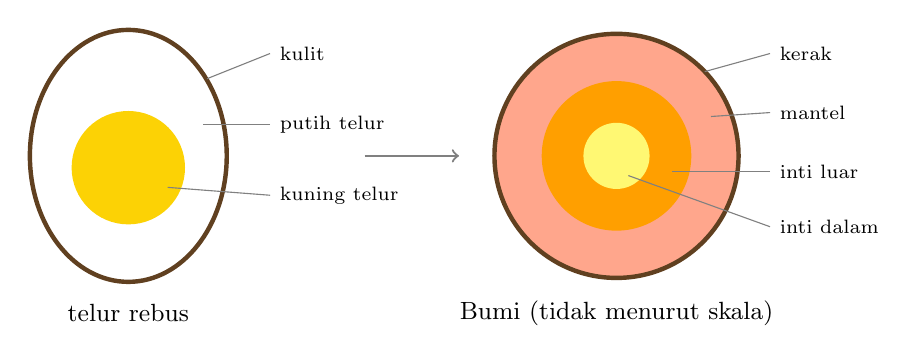
\begin{tikzpicture}
  % a boiled egg cut in half
  \begin{scope}
    \fill[white] (0,0) ellipse (1.25 and 1.6);
    \draw[brown!50!black, line width=1.6pt] (0,0) ellipse (1.25 and 1.6);
    \fill[yellow!70!orange] (0,-0.15) circle (0.72);
    \node[font=\scriptsize, anchor=west] (s) at (1.8,1.3) {kulit};
    \draw[gray] (s.west) -- (1.0,0.98);
    \node[font=\scriptsize, anchor=west] (w) at (1.8,0.4) {putih telur};
    \draw[gray] (w.west) -- (0.95,0.4);
    \node[font=\scriptsize, anchor=west] (y) at (1.8,-0.5) {kuning telur};
    \draw[gray] (y.west) -- (0.5,-0.4);
    \node[font=\small] at (0,-2.0) {telur rebus};
  \end{scope}
  \draw[->, thick, gray] (3.0,0) -- (4.2,0);
  % the Earth, not to scale
  \begin{scope}[xshift=6.2cm]
    \fill[orange!45!red!45] (0,0) circle (1.55);
    \fill[orange!75!yellow] (0,0) circle (0.95);
    \fill[yellow!55] (0,0) circle (0.42);
    \draw[brown!50!black, line width=1.6pt] (0,0) circle (1.55);
    \node[font=\scriptsize, anchor=west] (c) at (1.95,1.3) {kerak};
    \draw[gray] (c.west) -- (1.12,1.07);
    \node[font=\scriptsize, anchor=west] (m) at (1.95,0.55) {mantel};
    \draw[gray] (m.west) -- (1.2,0.5);
    \node[font=\scriptsize, anchor=west] (o) at (1.95,-0.2) {inti luar};
    \draw[gray] (o.west) -- (0.7,-0.2);
    \node[font=\scriptsize, anchor=west] (i) at (1.95,-0.9) {inti dalam};
    \draw[gray] (i.west) -- (0.15,-0.25);
    \node[font=\small] at (0,-2.0) {Bumi (tidak menurut skala)};
  \end{scope}
\end{tikzpicture}

{\small Bumi dibandingkan dengan telur rebus. Berbeda dengan kuning telur,
\omterm{def:g6:inside-the-earth:layers}{inti} Bumi terdiri atas dua bagian. Pada gambar ini \omterm{def:g6:inside-the-earth:layers}{keraknya} digambar
terlalu tebal; gambar menurut skala menyusul berikutnya.}
% ledger: usgs:layers-egg
\end{omfigure}

\begin{definition}[Lapisan-lapisan Bumi]\label{def:g6:inside-the-earth:layers}
Bumi tersusun dari tiga lapisan utama, dari permukaan sampai ke pusat:
\begin{itemize}
  \item \emph{kerak}\index{kerak}, lapisan luar yang tipis dari \omterm{def:g3:stones-pebbles-sand:rock}{batuan} padat,
        yang tebalnya beberapa kilometer sampai beberapa puluh kilometer;
  \item \emph{mantel}\index{mantel}, lapisan tebal dari \omterm{def:g3:stones-pebbles-sand:rock}{batuan} padat yang
        panas dan bermassa jenis tinggi, sampai kedalaman kira-kira 2900~km;
  \item \emph{inti}\index{inti}, yang tersusun dari logam, terutama besi
        dengan sedikit nikel, dari kedalaman kira-kira 2900~km sampai ke
        pusat. Inti terdiri atas dua bagian: \emph{inti luar}\index{inti luar},
        yang cair, dan \emph{inti dalam}\index{inti dalam}, sebuah bola padat
        di pusat, yang jari-jarinya kira-kira 1220~km.
\end{itemize}
% ledger: usgs:layers-egg, usgs:crust-thickness, data:prem, earth:Rmean
\end{definition}

Gambar di bawah ini menunjukkan lapisan-lapisan itu \emph{menurut skala},
dengan batas-batas yang diukur oleh gelombang \omterm{def:g4:volcanoes-earthquakes-first-look:earthquake}{gempa bumi}.

\begin{omfigure}
\pgfplotstableread{figdata/out/grade-6-earth_layers-disc.dat}\disctab
\pgfplotstablegetelem{0}{r_cm}\of\disctab \let\rE\pgfplotsretval
\pgfplotstablegetelem{1}{r_cm}\of\disctab \let\rOC\pgfplotsretval
\pgfplotstablegetelem{2}{r_cm}\of\disctab \let\rIC\pgfplotsretval
\begin{minipage}[c]{0.43\linewidth}\centering
\begin{tikzpicture}
  \fill[orange!45!red!45] (0,0) circle (\rE cm);
  \fill[orange!75!yellow] (0,0) circle (\rOC cm);
  \fill[yellow!55] (0,0) circle (\rIC cm);
  \draw[brown!50!black, line width=0.45pt] (0,0) circle (\rE cm);
  
  \draw[gray, thin] (-0.25,\rE) rectangle (0.25,\rE-0.12);
  
  \node[font=\scriptsize, align=center, inner sep=0pt] at (0,0) {inti\\ dalam};
  \node[font=\scriptsize, align=center] at (0,1.03) {inti\\ luar};
  \node[font=\scriptsize] at (0,2.12) {mantel};
  \draw[<-, font=\scriptsize] (1.98,1.98) -- (2.3,2.75) node[above, align=center] {kerak\\ (setipis rambut)};
\end{tikzpicture}
\end{minipage}\hfill
\begin{minipage}[c]{0.55\linewidth}\centering
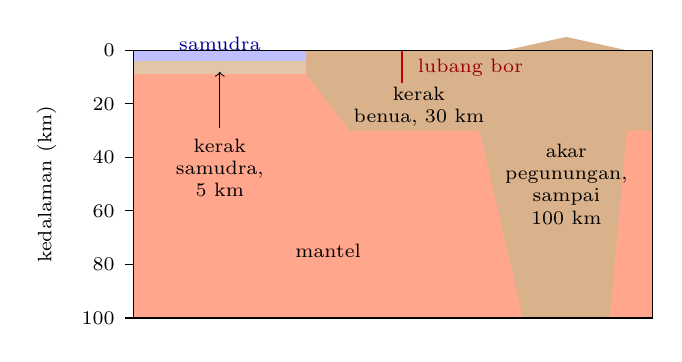
\begin{tikzpicture}[yscale=0.034, xscale=0.55]
  % the top 100 km enlarged: ocean on the left, continent and a range on the right
  \fill[orange!45!red!45] (0,0) rectangle (12,-100);
  \fill[blue!25] (0,0) rectangle (4,-4);
  \fill[brown!45] (0,-4) rectangle (4,-9);                 % oceanic crust 5 km
  \fill[brown!60] (4,0) -- (4,-9) -- (5,-30) -- (8,-30) -- (9,-100) -- (11,-100) -- (11.4,-30) -- (12,-30) -- (12,0) -- cycle;
  \fill[brown!60] (8.6,0) -- (10,5) -- (11.4,0) -- cycle;   % the range (not to scale above ground)
  \draw[red!75!black, line width=0.8pt] (6.2,0) -- (6.2,-12.262);
  \draw[thin] (0,0) rectangle (12,-100);
  \foreach \y in {0,-20,-40,-60,-80,-100} \draw (0,\y) -- (-0.2,\y) node[left, font=\scriptsize] {\pgfmathparse{-\y}\pgfmathprintnumber{\pgfmathresult}};
  \node[font=\scriptsize, rotate=90] at (-2.0,-50) {kedalaman (km)};
  \node[font=\scriptsize, align=center] at (2,-44) {kerak\\ samudra,\\ 5~km};
  \draw[->, thin] (2,-29) -- (2,-8);
  \node[font=\scriptsize, align=center] at (6.6,-21) {kerak\\ benua, 30~km};
  \node[font=\scriptsize, align=center] at (10.0,-50) {akar\\ pegunungan,\\ sampai\\ 100~km};
  \node[font=\scriptsize, anchor=west, red!60!black] at (6.35,-6.5) {lubang bor};
  \node[font=\scriptsize] at (4.5,-75) {mantel};
  \node[font=\scriptsize, blue!60!black] at (2,2.5) {samudra};
\end{tikzpicture}
\end{minipage}

\smallskip
{\small Kiri: Bumi dibelah, menurut skala; kotak kelabu kecil di bagian atas
menandai bagian yang diperbesar di sebelah kanan. Kanan: 100~km teratas,
diperbesar kira-kira 60~kali: \omterm{def:g6:inside-the-earth:layers}{kerak} yang tipis di bawah \omterm{def:g2:water-on-earth:ocean}{samudra}, \omterm{def:g6:inside-the-earth:layers}{kerak} yang
lebih tebal di bawah \omterm{def:g3:continents-and-oceans:continent}{benua}, paling tebal di bawah \omterm{def:g4:world-physical-map:range}{pegunungan} yang tinggi;
lubang bor pemegang rekor berwarna merah.}
% ledger: data:prem, earth:Rmean, usgs:crust-thickness, sciam:kola-depth (figdata/grade-6/earth_layers.py)
\end{omfigure}

\begin{center}\small
\begin{tabular}{|l|c|c|c|l|}
\hline
\textbf{lapisan} & \textbf{dari (km)} & \textbf{sampai (km)} & \textbf{tebal (km)} & \textbf{tersusun dari} \\
\hline
\omterm{def:g6:inside-the-earth:layers}{kerak} & 0 & 5 sampai 100 & 5 sampai 100 & \omterm{def:g3:stones-pebbles-sand:rock}{batuan} padat \\
\omterm{def:g6:inside-the-earth:layers}{mantel} & dasar \omterm{def:g6:inside-the-earth:layers}{kerak} & 2891 & kira-kira 2860 & \omterm{def:g3:stones-pebbles-sand:rock}{batuan} padat, sangat panas \\
\omterm{def:g6:inside-the-earth:layers}{inti luar} & 2891 & 5150 & kira-kira 2260 & logam cair \\
\omterm{def:g6:inside-the-earth:layers}{inti dalam} & 5150 & 6371 (pusat) & kira-kira 1220 & logam padat \\
\hline
\end{tabular}
\end{center}
% ledger: data:prem, usgs:crust-thickness, usgs:layers-egg, earth:Rmean (figdata/grade-6/earth_layers.py, main table)

\textbf{\omterm{def:g6:inside-the-earth:layers}{Kerak}} adalah satu-satunya lapisan yang dapat kita injak dan gali.
\omterm{def:g6:inside-the-earth:layers}{Kerak} sangat tipis dibandingkan dengan lapisan lainnya: di bawah \omterm{def:g2:water-on-earth:ocean}{samudra},
tebalnya hanya kira-kira 5~km; di bawah \omterm{def:g3:continents-and-oceans:continent}{benua}, rata-rata kira-kira 30~km; di
bawah \omterm{def:g4:world-physical-map:range}{pegunungan} yang tinggi seperti \omterm{def:g4:world-physical-map:range}{Pegunungan} Alpen, dasarnya dapat
mencapai kedalaman 100~km, seperti akar gigi. Bahkan lubang bor pemegang
rekor, sedalam 12.3~km, menembus kurang dari separuh \omterm{def:g6:inside-the-earth:layers}{kerak} \omterm{def:g3:continents-and-oceans:continent}{benua} yang
rata-rata. Pada gambar menurut skala, \omterm{def:g6:inside-the-earth:layers}{kerak} lebih tipis daripada garis yang
mengelilingi cakram itu.
% ledger: usgs:crust-thickness, sciam:kola-depth

\textbf{\omterm{def:g6:inside-the-earth:layers}{Mantel}} adalah lapisan yang paling tebal: dari dasar \omterm{def:g6:inside-the-earth:layers}{kerak} sampai
2891~km, kira-kira 45~\% dari perjalanan menuju pusat. \omterm{def:g3:stones-pebbles-sand:rock}{Batuannya} padat,
tetapi sangat panas dan lebih padat massanya daripada \omterm{def:g3:stones-pebbles-sand:rock}{batuan} \omterm{def:g6:inside-the-earth:layers}{kerak}. Selama
jutaan tahun, \omterm{def:g3:stones-pebbles-sand:rock}{batuan} panas di sebagian \omterm{def:g6:inside-the-earth:layers}{mantel} dapat merayap dengan sangat
lambat, seperti adonan yang sangat kaku.
% ledger: data:prem, usgs:layers-egg, usgs:lithosphere-80km

\textbf{\omterm{def:g6:inside-the-earth:layers}{Inti}} dimulai pada 2891~km dan menerus sampai ke pusat. \omterm{def:g6:inside-the-earth:layers}{Inti} tidak
tersusun dari \omterm{def:g3:stones-pebbles-sand:rock}{batuan}, melainkan dari logam: paduan besi dan nikel, yang
massa jenisnya hampir dua kali massa jenis \omterm{def:g6:inside-the-earth:layers}{mantel}. Bagian luarnya
\emph{cair}: \omterm{def:g2:water-on-earth:ocean}{samudra} logam leleh yang dalamnya lebih dari 2000~km. Bagian
dalamnya, dari 5150~km sampai ke pusat, adalah bola logam yang
\emph{padat}, dengan jari-jari kira-kira 1220~km: kira-kira 70~\% lebar
Bulan. Ketika Bumi berputar, logam cair di \omterm{def:g6:inside-the-earth:layers}{inti luar} bergerak, dan gerakan
inilah yang menghasilkan medan magnet Bumi, yang menggerakkan jarum
kompas.
% ledger: data:prem, usgs:layers-egg, earth:Rmean, planet:Moon.diameter

Makin dalam, makin besar massa jenisnya. Air mempunyai massa jenis 1~gram
per sentimeter kubik: massa jenis \omterm{def:g3:stones-pebbles-sand:rock}{batuan} \omterm{def:g6:inside-the-earth:layers}{kerak} 2.6 sampai 2.9 kali massa
jenis air, \omterm{def:g3:stones-pebbles-sand:rock}{batuan} di dasar \omterm{def:g6:inside-the-earth:layers}{mantel} lebih dari 5~kali, dan logam di pusat
kira-kira 13~kali (lihat grafik di bawah ini). Bahan-bahan yang paling
berat berada di pusat dan yang paling ringan di atas: Bumi tersusun
berurutan, dari \omterm{def:g6:inside-the-earth:layers}{kerak} yang ringan sampai \omterm{def:g6:inside-the-earth:layers}{inti} logam yang berat.
% ledger: data:prem


\begin{omfigure}
\begin{tikzpicture}
  \begin{axis}[omrecord, width=0.86\linewidth, height=5.4cm,
      xmin=0, xmax=6371, ymin=0, ymax=14,
      xlabel={kedalaman di bawah permukaan (km)},
      ylabel={massa jenis (g per cm$^3$)},
      xtick={0,1000,2000,3000,4000,5000,6000},
      scaled x ticks=false, x tick label style={/pgf/number format/1000 sep={}},
      clip=false]
    \fill[orange!45!red!20] (axis cs:24.4,0) rectangle (axis cs:2891,14);
    \fill[orange!75!yellow!35] (axis cs:2891,0) rectangle (axis cs:5149.5,14);
    \fill[yellow!30] (axis cs:5149.5,0) rectangle (axis cs:6371,14);
    \addplot[very thick, black] table[x=depth_km, y=rho] {figdata/out/grade-6-earth_layers-profile.dat};
    \node[font=\scriptsize] at (axis cs:1450,12.5) {mantel};
    \node[font=\scriptsize] at (axis cs:4020,4.5) {inti luar};
    \node[font=\scriptsize] at (axis cs:5760,4.5) {inti dalam};
    \node[font=\scriptsize, align=left, anchor=west] at (axis cs:80,1.4) {kerak: 2.6 sampai 2.9};
  \end{axis}
\end{tikzpicture}

{\small Massa jenis Bumi pada setiap kedalaman, menurut sebuah model acuan
yang dibangun dari pengukuran \omterm{def:g4:volcanoes-earthquakes-first-look:earthquake}{gempa bumi}. Massa jenisnya melompat dari
kira-kira 5.6 menjadi kira-kira 9.9~g per cm$^3$ di tempat \omterm{def:g3:stones-pebbles-sand:rock}{batuan} \omterm{def:g6:inside-the-earth:layers}{mantel}
berganti menjadi logam \omterm{def:g6:inside-the-earth:layers}{inti}.}
% ledger: data:prem (figdata/grade-6/earth_layers.py, part profile)
\end{omfigure}

\begin{inthelab}[Lapisan-lapisan di dalam gelas (di kelas, bersama guru)]
Guru menuangkan, perlahan-lahan dan berturut-turut, ke dalam sebuah gelas
tinggi: sedikit madu, sedikit air yang diwarnai dengan setetes tinta, dan
sedikit minyak goreng. Apa pun urutan penuangannya, setelah beberapa saat
madu berada di dasar, air di tengah, dan minyak di atas: setiap cairan
mengendap di bawah cairan yang lebih ringan dan di atas cairan yang lebih
padat massanya. Jika dikocok, isi gelas menjadi keruh; jika dibiarkan,
isinya tersusun kembali. Bumi berlapis dengan cara yang sama: bahan yang
massa jenisnya paling besar, yaitu logam \omterm{def:g6:inside-the-earth:layers}{inti}, berada di pusat, dan \omterm{def:g3:stones-pebbles-sand:rock}{batuan}
yang paling ringan berada di atas.
\end{inthelab}


\begin{remark}[Seberapa tipis kerak itu?]\label{rem:g6:inside-the-earth:thin-crust}
Pada \omterm{def:g3:continents-and-oceans:globe}{bola dunia} sekolah yang lebarnya 30~cm, \omterm{def:g6:inside-the-earth:layers}{kerak} \omterm{def:g3:continents-and-oceans:continent}{benua} (30~km) akan
setebal kira-kira 0.7~milimeter, dan \omterm{def:g6:inside-the-earth:layers}{kerak} \omterm{def:g2:water-on-earth:ocean}{samudra} (5~km) kira-kira setebal
selembar kertas. \omterm{def:g6:inside-the-earth:layers}{Kerak} itu kurang dari setengah persen jari-jari Bumi:
$30 \div 6371 \approx 0.0047$, yaitu 0.47~\%.
% ledger: usgs:crust-thickness, earth:Rmean
\end{remark}

\section{Bagaimana gelombang gempa bumi menceritakan sisanya}\label{sec:g6:inside-the-earth:waves}

Jika tidak ada seorang pun yang pernah masuk lebih dalam dari 12~km,
bagaimana kita dapat menggambar \omterm{def:g6:inside-the-earth:layers}{inti} Bumi? Jawabannya datang dari \omterm{def:g4:volcanoes-earthquakes-first-look:earthquake}{gempa
bumi}. Ketika \omterm{def:g4:volcanoes-earthquakes-first-look:earthquake}{gempa bumi} mengguncang tanah, gelombang-gelombang memancar ke
segala arah dan merambat \emph{menembus} seluruh Bumi, seperti bunyi ketukan
merambat menembus dinding. Alat-alat ukur di banyak tempat di seluruh dunia
mencatat waktu tibanya setiap gelombang (kamu akan mengenalnya dalam
\cref{ch:g7:earthquakes}).
% ledger: data:prem

Gelombang tidak merambat dengan kecepatan yang sama di setiap bahan. Ketika
sampai di batas antara dua lapisan, kecepatannya berubah tiba-tiba: ada
gelombang yang memantul kembali, ada yang membelok ketika menyeberang, agak
mirip cahaya yang masuk ke dalam air. Dengan mengukur waktu tempuh gelombang
dari banyak \omterm{def:g4:volcanoes-earthquakes-first-look:earthquake}{gempa bumi}, di stasiun-stasiun di seluruh dunia, para ilmuwan
telah menemukan letak batas-batas ini, dan lapisan mana yang padat atau
cair. Para ahli seismologi menyebut kedua jenis gelombang utama
\emph{gelombang P} (yang lebih cepat, yang mendorong dan menarik \omterm{def:g3:stones-pebbles-sand:rock}{batuan}) dan
\emph{gelombang S} (yang lebih lambat, yang mengguncangnya ke samping); jilid
berikutnya mempelajarinya dengan saksama. Gelombang S mempunyai satu sifat
yang luar biasa: gelombang ini tidak dapat merambat melalui zat cair.

\begin{omfigure}
\begin{tikzpicture}
  \begin{axis}[omrecord, width=0.86\linewidth, height=5.4cm,
      xmin=0, xmax=6371, ymin=0, ymax=14.5,
      xlabel={kedalaman di bawah permukaan (km)},
      ylabel={kecepatan gelombang (km per detik)},
      xtick={0,1000,2000,3000,4000,5000,6000},
      scaled x ticks=false, x tick label style={/pgf/number format/1000 sep={}},
      clip=false]
    \fill[orange!45!red!20] (axis cs:24.4,0) rectangle (axis cs:2891,14.5);
    \fill[orange!75!yellow!35] (axis cs:2891,0) rectangle (axis cs:5149.5,14.5);
    \fill[yellow!30] (axis cs:5149.5,0) rectangle (axis cs:6371,14.5);
    \addplot[very thick, blue!70!black] table[x=depth_km, y=vp] {figdata/out/grade-6-earth_layers-profile.dat};
    \addplot[very thick, red!75!black] table[x=depth_km, y=vs] {figdata/out/grade-6-earth_layers-profile.dat};
    \node[font=\scriptsize, blue!70!black, anchor=south] at (axis cs:1300,12.9) {gelombang P (lebih cepat)};
    \node[font=\scriptsize, red!75!black, anchor=north] at (axis cs:1500,6.1) {gelombang S (lebih lambat)};
    \node[font=\scriptsize, red!75!black, align=center, fill=white, fill opacity=0.8, text opacity=1] at (axis cs:4020,1.9) {gelombang S: 0\\ (cair)};
    \node[font=\scriptsize] at (axis cs:4020,13.6) {inti luar};
    \node[font=\scriptsize] at (axis cs:5760,13.6) {inti dalam};
    \node[font=\scriptsize] at (axis cs:1450,1.5) {mantel};
  \end{axis}
\end{tikzpicture}

{\small Kecepatan kedua jenis gelombang \omterm{def:g4:volcanoes-earthquakes-first-look:earthquake}{gempa bumi} pada setiap kedalaman,
menurut model acuan yang sama. Di \omterm{def:g6:inside-the-earth:layers}{inti luar}, gelombang S berhenti:
kecepatannya nol, karena \omterm{def:g6:inside-the-earth:layers}{inti luar} itu cair.}
% ledger: data:prem (figdata/grade-6/earth_layers.py, part profile)
\end{omfigure}

Membaca grafik dari kiri ke kanan: di \omterm{def:g6:inside-the-earth:layers}{mantel}, kedua jenis gelombang makin
cepat seiring bertambahnya kedalaman. Pada 2891~km, gelombang S menghilang
dan gelombang P tiba-tiba melambat: inilah bagian atas \omterm{def:g6:inside-the-earth:layers}{inti luar} yang cair.
Pada 5150~km, gelombang P bertambah cepat lagi dan gelombang S muncul
kembali: inilah \omterm{def:g6:inside-the-earth:layers}{inti dalam} yang padat.
% ledger: data:prem

\begin{history}[Inge Lehmann dan inti dalam]
\begin{minipage}[c]{0.72\linewidth}
Pada awal tahun 1930-an, para ahli seismologi mengira bahwa Bumi terdiri
atas dua lapisan: \omterm{def:g6:inside-the-earth:layers}{mantel} padat yang mengelilingi \omterm{def:g6:inside-the-earth:layers}{inti} cair. Ahli seismologi
Denmark, Inge Lehmann, mempelajari gelombang dari sebuah \omterm{def:g4:volcanoes-earthquakes-first-look:earthquake}{gempa bumi} kuat yang
melanda Selandia Baru pada tahun 1929, yang tercatat di stasiun-stasiun yang
jauh. Ada gelombang yang tiba di tempat yang seharusnya sama sekali tidak
didatangi gelombang jika \omterm{def:g6:inside-the-earth:layers}{intinya} cair seluruhnya. Dalam sebuah artikel
tahun 1936, yang berjudul singkat ``P\,$'$'', ia mengusulkan sebuah
penjelasan: di dalam \omterm{def:g6:inside-the-earth:layers}{inti} yang cair terdapat \emph{\omterm{def:g6:inside-the-earth:layers}{inti dalam} yang padat}
yang lebih kecil, yang memantulkan gelombang-gelombang itu. Dengan rendah
hati ia menulis bahwa datanya ``sama sekali tidak memadai'' untuk memastikan
hal itu, tetapi tafsiran itu ``tampaknya mungkin'', dan ia meminta para
peneliti lain untuk mengujinya. Mereka melakukannya, dan sekarang \omterm{def:g6:inside-the-earth:layers}{inti
dalam} yang padat menjadi bagian dari setiap model acuan Bumi, seperti model
yang dipakai dalam grafik-grafik bab ini.
% ledger: nbi:lehmann-1936
\end{minipage}\hfill
\begin{minipage}[c]{0.24\linewidth}\centering
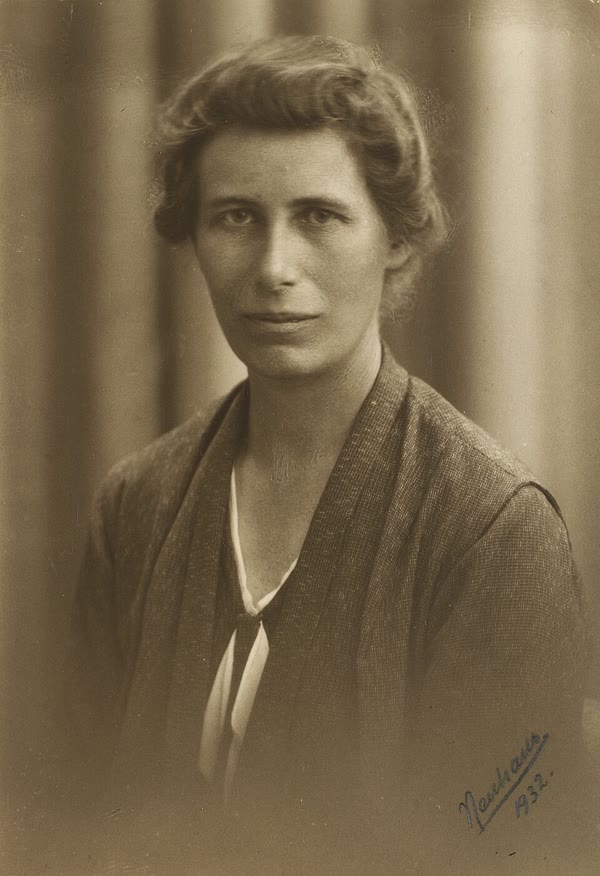
\includegraphics[width=\linewidth]{images/book1/g6-inge-lehmann.jpg}\\[2pt]
{\footnotesize Inge Lehmann pada tahun 1932. (Foto karya Even Neuhaus, domain
publik, melalui Wikimedia Commons.)}
% ledger: commons:inge-lehmann
\end{minipage}
\end{history}

\section{Makin dalam, makin panas}

Setiap tambang yang dalam dan setiap lubang bor yang dalam menunjukkan hal
yang sama: makin dalam kita masuk, makin panas \omterm{def:g3:stones-pebbles-sand:rock}{batuannya}. Di tambang
terdalam, dinding \omterm{def:g3:stones-pebbles-sand:rock}{batuannya} mencapai kira-kira 60~derajat Celsius, lebih
dari 4~km di bawah tanah; di dasar lubang bor pemegang rekor, 12.3~km di
bawah tanah, suhu \omterm{def:g3:stones-pebbles-sand:rock}{batuannya} kira-kira 180~derajat.
% ledger: gwr:deepest-mine, sciam:kola-180C

Di dekat permukaan, suhu naik dengan laju yang cukup tetap. Di Amerika
Serikat, para ilmuwan mengumpulkan hasil pengukuran dari 284 lubang bor,
yang kebanyakan lebih dalam dari 600~m. Rata-rata, suhunya naik
\textbf{29~derajat untuk setiap kilometer} kedalaman: kira-kira 25~derajat
per kilometer di bagian timur negara itu dan 34 di bagian barat. Akan
tetapi, lajunya sangat berbeda dari satu tempat ke tempat lain: di
lubang-lubang itu, lajunya berkisar dari 6 sampai 69~derajat per kilometer.
% ledger: usgs:gradient-29

\begin{omfigure}
\begin{tikzpicture}
  \begin{axis}[omrecord, omdepth, width=0.78\linewidth, height=5.6cm,
      xmin=0, xmax=160, ymin=0, ymax=2,
      xlabel={suhu batuan ($^\circ$C)},
      ylabel={kedalaman (km)},
      ytick={0,0.5,1,1.5,2},
      yticklabel style={/pgf/number format/fixed},
      legend pos=north east, legend cell align=left,
            legend style={font=\scriptsize},
      clip=false]
    \addplot[forget plot, name path=lo, thin, gray] table[x=t_low, y=depth_km] {figdata/out/grade-6-earth_layers-geotherm.dat};
    \addplot[forget plot, name path=hi, thin, gray] table[x=t_high, y=depth_km] {figdata/out/grade-6-earth_layers-geotherm.dat};
    \addplot[forget plot, gray!20] fill between[of=lo and hi];
    \addplot[forget plot, thick, blue!70!black] table[x=t_east, y=depth_km] {figdata/out/grade-6-earth_layers-geotherm.dat};
    \addplot[forget plot, very thick, black] table[x=t_mean, y=depth_km] {figdata/out/grade-6-earth_layers-geotherm.dat};
    \addplot[forget plot, thick, red!75!black] table[x=t_west, y=depth_km] {figdata/out/grade-6-earth_layers-geotherm.dat};
    \addlegendimage{area legend, fill=gray!20, draw=gray}
    \addlegendentry{6 sampai 69 $^\circ$C per km: semua lubang}
    \addlegendimage{thick, blue!70!black}\addlegendentry{25 $^\circ$C per km: timur}
    \addlegendimage{very thick, black}\addlegendentry{29 $^\circ$C per km: rata-rata}
    \addlegendimage{thick, red!75!black}\addlegendentry{34 $^\circ$C per km: barat}
  \end{axis}
\end{tikzpicture}

{\small Suhu terhadap kedalaman (ke bawah) untuk tanah yang suhu awalnya
15~$^\circ$C, pada laju rata-rata (29, hitam), rata-rata bagian timur dan
barat (25 dan 34), dan seluruh rentang yang terukur (6 sampai 69, pita
kelabu). Pengukurannya mencapai kira-kira 2~km.}
% ledger: usgs:gradient-29, planet:Earth.Tmean (figdata/grade-6/earth_layers.py, part geotherm)
\end{omfigure}

\begin{method}[Suhu pada suatu kedalaman]\label{met:g6:inside-the-earth:temperature}
\begin{enumerate}
  \item Ambillah suhu tanah di dekat permukaan.
  \item Kalikan kedalamannya, dalam kilometer, dengan lajunya, dalam derajat
        per kilometer: hasilnya adalah besarnya kenaikan suhu.
  \item Jumlahkan keduanya. Pakailah cara ini hanya pada rentang tempat laju
        itu diukur: beberapa kilometer.
\end{enumerate}
\end{method}

\begin{example}[Dua kilometer di bawah tanah]\label{ex:g6:inside-the-earth:two-km}
Suhu tanahnya 15~$^\circ$C dan lajunya 29~derajat per kilometer. Pada 2~km:
$2 \times 29 = 58$ derajat lebih panas, jadi $15 + 58 = 73~^\circ$C: lebih
panas daripada air mandi yang paling panas, dan sudah terlalu panas untuk
disentuh.
% ledger: usgs:gradient-29, planet:Earth.Tmean
\end{example}

Dapatkah laju yang sama dipakai sampai ke pusat? Tidak. Dengan 29~derajat
per kilometer, pusat Bumi akan bersuhu kira-kira 185\,000~derajat, dan itu
mustahil: laju yang diukur pada kilometer-kilometer pertama tidak berlaku
jauh di bawah, tempat kenaikan suhu pasti jauh lebih lambat. Para ilmuwan
memperkirakan suhu \omterm{def:g6:inside-the-earth:layers}{inti} dengan cara lain: di laboratorium, mereka menjepit
butiran besi yang sangat kecil di antara dua intan, sampai tekanannya
jutaan kali tekanan udara, lalu memanaskannya dengan laser sampai meleleh.
Dengan cara ini, mereka menemukan bahwa di tepi \omterm{def:g6:inside-the-earth:layers}{inti dalam} yang padat
suhunya kira-kira \textbf{6000~derajat Celsius}, tetapi besi di \omterm{def:g6:inside-the-earth:layers}{inti dalam}
tetap padat, karena tekanan di sana, kira-kira 3.3~juta kali tekanan udara,
mencegahnya meleleh.
% ledger: esrf:core-6000C, usgs:gradient-29

\begin{remark}[Panas, tetapi tetap padat]\label{rem:g6:inside-the-earth:pressure}
Jika suatu zat ditekan kuat-kuat, zat itu baru meleleh pada suhu yang lebih
tinggi. \omterm{def:g6:inside-the-earth:layers}{Mantel} sangat panas, tetapi tetap padat; \omterm{def:g6:inside-the-earth:layers}{inti luar} cair; \omterm{def:g6:inside-the-earth:layers}{inti
dalam}, yang lebih panas lagi, padat kembali, karena \omterm{def:g6:inside-the-earth:layers}{inti dalam} itulah yang
tertekan paling kuat. Meleleh atau tidaknya suatu zat bergantung pada suhu
\emph{dan} pada tekanan.
% ledger: esrf:core-6000C, data:prem
\end{remark}

\section{Latihan}

\begin{exercise}[$\star$]\label{exo:g6:inside-the-earth:1}
Sebutkan keempat lapisan Bumi secara berurutan, dari permukaan sampai ke
pusat. Lapisan manakah yang cair? Lapisan manakah yang tersusun dari logam?
\end{exercise}

\begin{exercise}[$\star$]\label{exo:g6:inside-the-earth:2}
Benar atau salah? Perbaiki kalimat yang salah.
(a) \omterm{def:g6:inside-the-earth:layers}{Kerak} lebih tebal di bawah \omterm{def:g2:water-on-earth:ocean}{samudra} daripada di bawah \omterm{def:g3:continents-and-oceans:continent}{benua}.
(b) \omterm{def:g6:inside-the-earth:layers}{Inti} tersusun dari \omterm{def:g3:stones-pebbles-sand:rock}{batuan}.
(c) \omterm{def:g6:inside-the-earth:layers}{Inti dalam} itu padat.
(d) Lubang bor terdalam yang pernah digali dalamnya kira-kira 12~km.
\end{exercise}

\begin{exercise}[$\star$]\label{exo:g6:inside-the-earth:3}
Gunakan tabel lapisan. (a) Pada kedalaman berapakah \omterm{def:g6:inside-the-earth:layers}{inti} dimulai? (b) Pada
kedalaman berapakah \omterm{def:g6:inside-the-earth:layers}{inti dalam} dimulai? (c) Berapa tebal \omterm{def:g6:inside-the-earth:layers}{inti luar}?
\end{exercise}

\begin{exercise}[$\star$]\label{exo:g6:inside-the-earth:4}
Bumi sering dibandingkan dengan telur rebus. Salin dan lengkapi: ``Kulit
telur seperti \ldots, putih telur seperti \ldots{} dan kuning telur seperti
\ldots{}. Akan tetapi, berbeda dengan kuning telur, \ldots{} terdiri atas
dua bagian: \ldots{} yang cair dan \ldots{} yang padat.''
\end{exercise}

\begin{exercise}[$\star\star$]\label{exo:g6:inside-the-earth:5}
Gunung Everest tingginya 8.849~km dan jari-jari Bumi 6371~km. Sebagai
persentase dari jari-jari, berapa tinggi Everest? Bulatkan sampai dua
tempat desimal. Apakah permukaan Bumi sangat bergelombang
jika dilihat dari jauh?
\end{exercise}

\begin{exercise}[$\star\star$]\label{exo:g6:inside-the-earth:6}
\omterm{def:g6:inside-the-earth:layers}{Kerak} \omterm{def:g3:continents-and-oceans:continent}{benua} rata-rata setebal 30~km dan \omterm{def:g6:inside-the-earth:layers}{kerak} \omterm{def:g2:water-on-earth:ocean}{samudra} 5~km. (a) Berapa kali
lebih tebal \omterm{def:g6:inside-the-earth:layers}{kerak} \omterm{def:g3:continents-and-oceans:continent}{benua}? (b) Di bawah \omterm{def:g4:world-physical-map:range}{pegunungan} yang tinggi, \omterm{def:g6:inside-the-earth:layers}{kerak} dapat
mencapai 100~km. Berapa kali lebih tebal daripada \omterm{def:g6:inside-the-earth:layers}{kerak} \omterm{def:g2:water-on-earth:ocean}{samudra}?
\end{exercise}

\begin{exercise}[$\star\star$]\label{exo:g6:inside-the-earth:7}
Di sebuah daerah, suhu tanahnya 12~$^\circ$C dan suhunya naik 25~derajat
per kilometer. Berapakah suhunya (a) pada 1~km, (b) pada 1.5~km, (c) pada
2~km?
\end{exercise}

\begin{exercise}[$\star\star$]\label{exo:g6:inside-the-earth:8}
Di sebuah lubang bor, suhu \omterm{def:g3:stones-pebbles-sand:rock}{batuan} 14~$^\circ$C di dekat permukaan dan
74~$^\circ$C pada kedalaman 2~km. Berapa derajat suhunya naik untuk setiap
kilometer? Apakah laju ini terletak di antara rata-rata bagian timur dan
barat dari pengukuran dalam bab ini?
\end{exercise}

\begin{exercise}[$\star\star$]\label{exo:g6:inside-the-earth:9}
Gunakan grafik kecepatan gelombang. (a) Berapa kecepatan gelombang P tepat
di atas \omterm{def:g6:inside-the-earth:layers}{inti}, pada kira-kira 2890~km, dan tepat di bawah bagian atas \omterm{def:g6:inside-the-earth:layers}{inti}?
(b) Di antara kedalaman berapakah kecepatan gelombang S bernilai nol?
(c) Apa yang diberitahukan hal ini kepada kita tentang lapisan itu?
\end{exercise}

\begin{exercise}[$\star\star$]\label{exo:g6:inside-the-earth:10}
Lubang bor pemegang rekor sedalam 12.3~km. (a) Berapa persen \omterm{def:g6:inside-the-earth:layers}{kerak} \omterm{def:g3:continents-and-oceans:continent}{benua}
yang rata-rata (30~km) yang ditembusnya? (b) Apakah lubang itu mencapai
\omterm{def:g6:inside-the-earth:layers}{mantel}?
\end{exercise}

\begin{exercise}[$\star\star\star$]\label{exo:g6:inside-the-earth:11}
Leo berkata: ``Di dekat permukaan, suhu naik 29~derajat per kilometer, jadi
di pusat, 6371~km di bawah, suhunya pasti $15 + 29 \times 6371$ derajat.''
(a) Hitunglah angka Leo. (b) Bandingkan angka itu dengan suhu yang
ditemukan di laboratorium untuk tepi \omterm{def:g6:inside-the-earth:layers}{inti dalam}. (c) Apa yang keliru dalam
penalaran Leo?
\end{exercise}

\begin{exercise}[$\star\star\star$]\label{exo:g6:inside-the-earth:12}
Bumi secara keseluruhan mempunyai massa jenis rata-rata kira-kira 5.5~gram
per sentimeter kubik (\cref{ch:g6:earth-a-planet}), tetapi \omterm{def:g3:stones-pebbles-sand:rock}{batuan} \omterm{def:g6:inside-the-earth:layers}{kerak}
massa jenisnya hanya 2.6 sampai 2.9. (a) Apa yang diberitahukan hal ini
kepada kita tentang bahan yang lebih dalam? (b) Gunakan grafik massa jenis:
di lapisan manakah massa jenisnya lebih dari 5.5 di semua tempat?
(c) Mengapa masuk akal bahwa logam yang berat terletak di pusat dan bukan
di permukaan?
\end{exercise}

\section{Soal: Perjalanan ke Pusat Bumi, Menurut Skala}

\begin{problem}[{Soal akhir pekan --- model Bumi selebar 2~meter: lapisan,
lubang terdalam, dan bagian dalam yang panas, digambar menurut skala}]
\label{pb:g6:inside-the-earth:1}
% ledger: earth:Rmean, data:prem, usgs:crust-thickness, sciam:kola-depth, tht:everest, usgs:gradient-29, gwr:deepest-mine, esrf:core-6000C
Untuk pameran sekolah, sebuah kelas membuat model Bumi yang dibelah dua,
sebesar mungkin: bidang datar dari setengah bola itu adalah cakram selebar
2~meter, yang dicat dengan lapisan-lapisannya. Semuanya harus menurut skala.
Pakailah: jari-jari Bumi 6371~km; bagian atas \omterm{def:g6:inside-the-earth:layers}{inti luar} 2891~km; bagian atas
\omterm{def:g6:inside-the-earth:layers}{inti dalam} 5150~km; \omterm{def:g6:inside-the-earth:layers}{kerak} \omterm{def:g3:continents-and-oceans:continent}{benua} 30~km; \omterm{def:g6:inside-the-earth:layers}{kerak} \omterm{def:g2:water-on-earth:ocean}{samudra} 5~km; Everest
8.849~km; lubang bor pemegang rekor 12.3~km.

\medskip
\noindent\textbf{Bagian I --- Modelnya.}
\begin{enumerate}
  \item Berapa diameter Bumi, dalam kilometer? Tuliskan diameter model itu
        dalam milimeter.
  \item Berapa kilometer Bumi yang sebenarnya diwakili oleh 1~milimeter pada
        model? (Bagilah diameter sebenarnya dengan diameter model.)
  \item Pada model, berapa tinggi Everest, dalam milimeter? Bulatkan sampai
        satu tempat desimal.
  \item Berapa dalam lubang bor pemegang rekor pada model? Bandingkan dengan
        jarak dari permukaan sampai ke pusat model.
\end{enumerate}

\medskip
\noindent\textbf{Bagian II --- Lapisan-lapisannya.}
\begin{enumerate}[resume]
  \item Pada jarak berapa di bawah permukaan model para siswa harus mengecat
        bagian atas \omterm{def:g6:inside-the-earth:layers}{inti luar}? Bulatkan ke milimeter terdekat.
  \item Pertanyaan yang sama untuk bagian atas \omterm{def:g6:inside-the-earth:layers}{inti dalam}. Berapa jari-jari
        \omterm{def:g6:inside-the-earth:layers}{inti dalam} pada model?
  \item Lapisan manakah yang mengambil tempat paling banyak di sepanjang
        jari-jari model: \omterm{def:g6:inside-the-earth:layers}{mantel}, \omterm{def:g6:inside-the-earth:layers}{inti luar}, atau \omterm{def:g6:inside-the-earth:layers}{inti dalam}? Berikan
        tebalnya pada model.
  \item Berapa tebal \omterm{def:g6:inside-the-earth:layers}{kerak} \omterm{def:g3:continents-and-oceans:continent}{benua} harus dicat? Bulatkan sampai satu tempat desimal. Apakah hal itu mudah dilakukan dengan kuas?
\end{enumerate}

\medskip
\noindent\textbf{Bagian III --- Bagian dalam yang panas.}
\begin{enumerate}[resume]
  \item Para siswa menuliskan suhu pada 2~km, dengan memakai tanah yang
        bersuhu 15~$^\circ$C dan 29~derajat per kilometer. Apa yang mereka
        tuliskan? Pada jarak berapa di bawah permukaan model letak 2~km itu?
  \item Tambang terdalam menembus lebih dari 4~km. Apakah tambang itu lebih
        dalam atau lebih dangkal daripada lubang bor pemegang rekor pada
        model? Kira-kira berapa milimeter selisihnya?
  \item Di dekat tepi \omterm{def:g6:inside-the-earth:layers}{inti dalam}, labelnya berbunyi ``kira-kira
        6000~$^\circ$C, padat''. Seorang pengunjung heran: mengapa \omterm{def:g6:inside-the-earth:layers}{inti luar}
        cair, tetapi \omterm{def:g6:inside-the-earth:layers}{inti dalam}, yang lebih panas lagi, padat?
  \item \omterm{def:g6:inside-the-earth:layers}{Kerak} \omterm{def:g2:water-on-earth:ocean}{samudra} adalah lapisan yang paling tipis. Berapa tebalnya pada
        model, dalam milimeter? Bulatkan sampai dua tempat desimal, dan bandingkan dengan tebal selembar kertas (kira-kira
        0.1~mm).
\end{enumerate}
\end{problem}
